% To create a slide, use the following:
% \begin{frame}{TITLE}
%     BODY
% \end{frame}

% To create a slide with a bullet list, use the following:
% \begin{frame}{TITLE}
%     \begin{itemize}
%         \item ITEM 1
%         \item ITEM 2
%     \end{itemize}    
% \end{frame}

% To create a slide with numbered list, use the following:
% \begin{frame}{TITLE}
%     \begin{enumerate}
%         \item ITEM 1
%         \item ITEM 2
%     \end{enumerate}
% \end{frame}

% To create a slide with a graphic:
% 1. Add the graphic to this folder (named picture.png)
% 2. Use the following:
% \begin{frame}{TITLE}
%     \centering
%     \includegraphics[height=0.7\textheight,width=0.7\textwidth,keepaspectratio]{images/}
% \end{frame}

% To create a slide with two columns, use the following:
\begin{frame}{Potting}
    \centering
    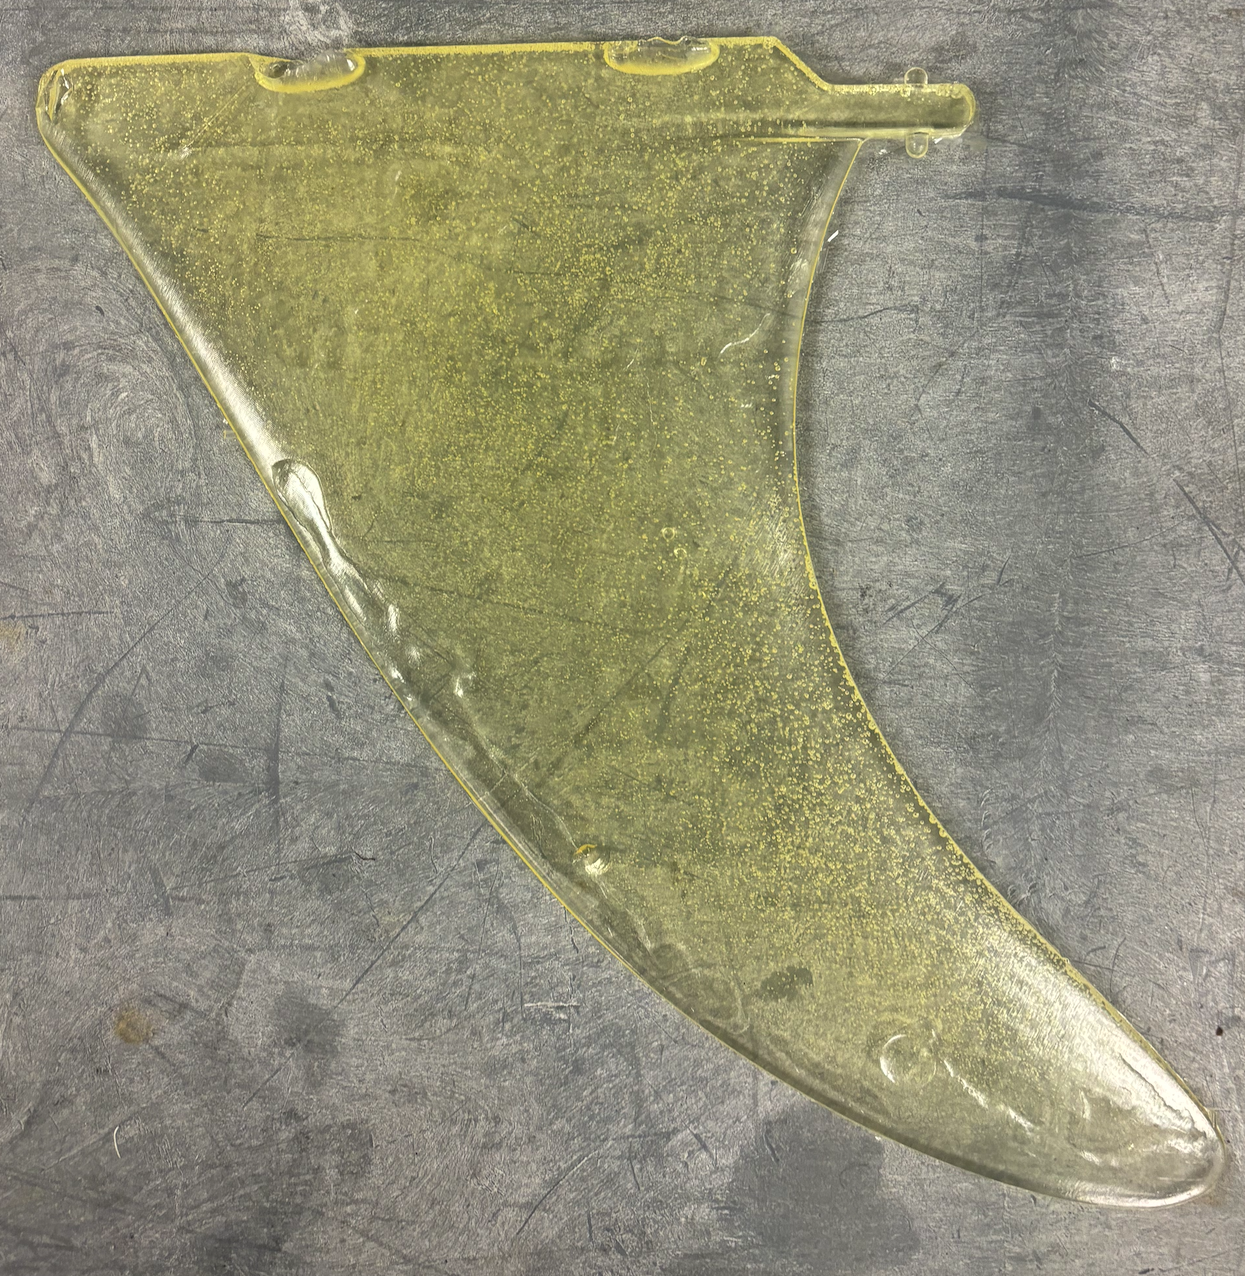
\includegraphics[height=0.8\textheight,width=0.8\textwidth,keepaspectratio]{images/Epoxy_fin.png}
\end{frame}
\begin{frame}{PCB Debugging}
    \centering
    \includegraphics[height=0.8\textheight,width=0.8\textwidth,keepaspectratio]{images/pcb_hw_mods.png}
\end{frame}
\begin{frame}{PCB Work}
    \begin{columns}
        \begin{column}{0.5\textwidth}
            No IMU Response
            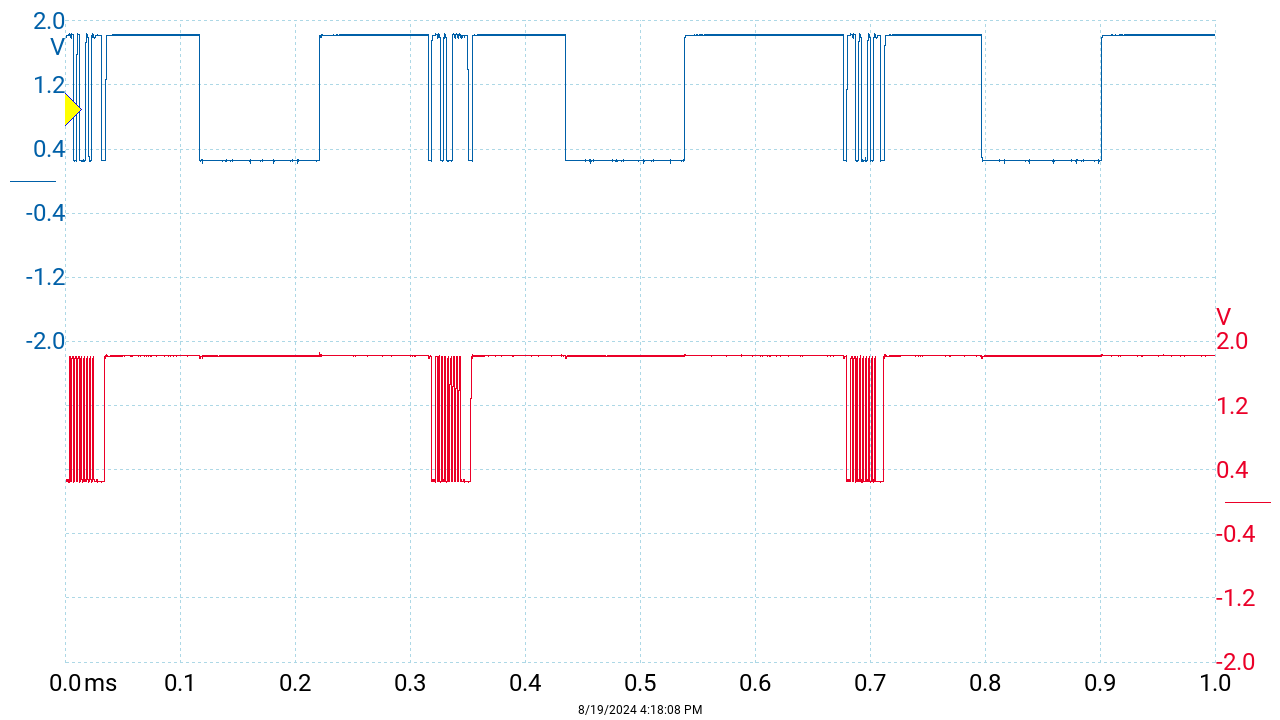
\includegraphics[height=1\textheight,width=1\textwidth,keepaspectratio]{images/IMU_SDA_SCL_NoData.png}
        \end{column}
        \begin{column}{0.5\textwidth}
            Capacitance Issues
            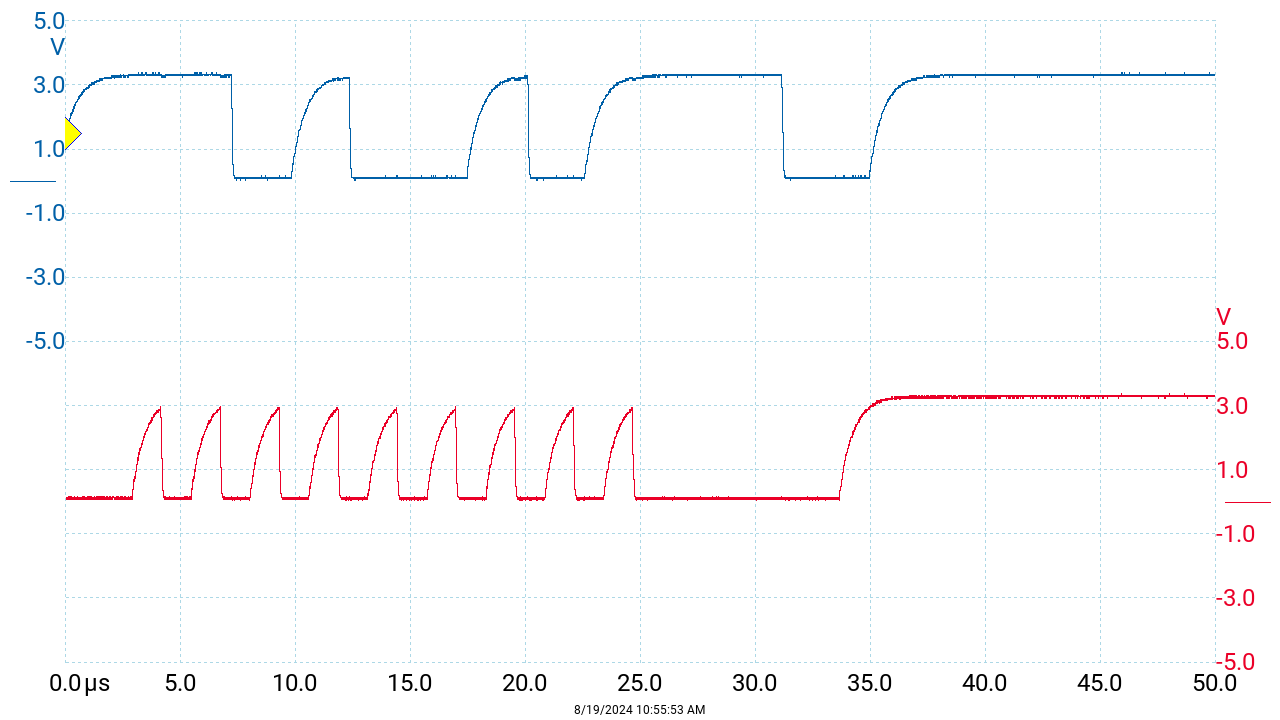
\includegraphics[height=1\textheight,width=1\textwidth,keepaspectratio]{images/PreResistorChange_Both.png}
        \end{column}
    \end{columns}
\end{frame}

\begin{frame}{Software Updates}
    Creating testing suite, code review Wednesday
    \begin{columns}
        \begin{column}{0.5\textwidth}
            
            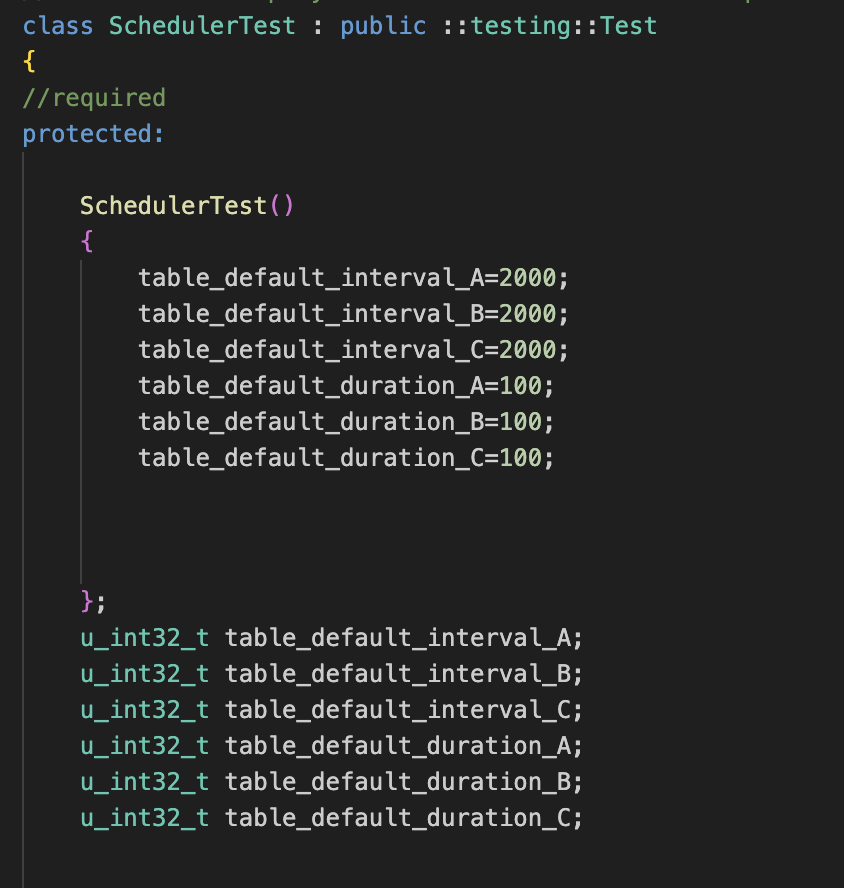
\includegraphics[height=1\textheight,width=1\textwidth,keepaspectratio]{images/testClass.png}
        \end{column}
        \begin{column}{0.5\textwidth}
            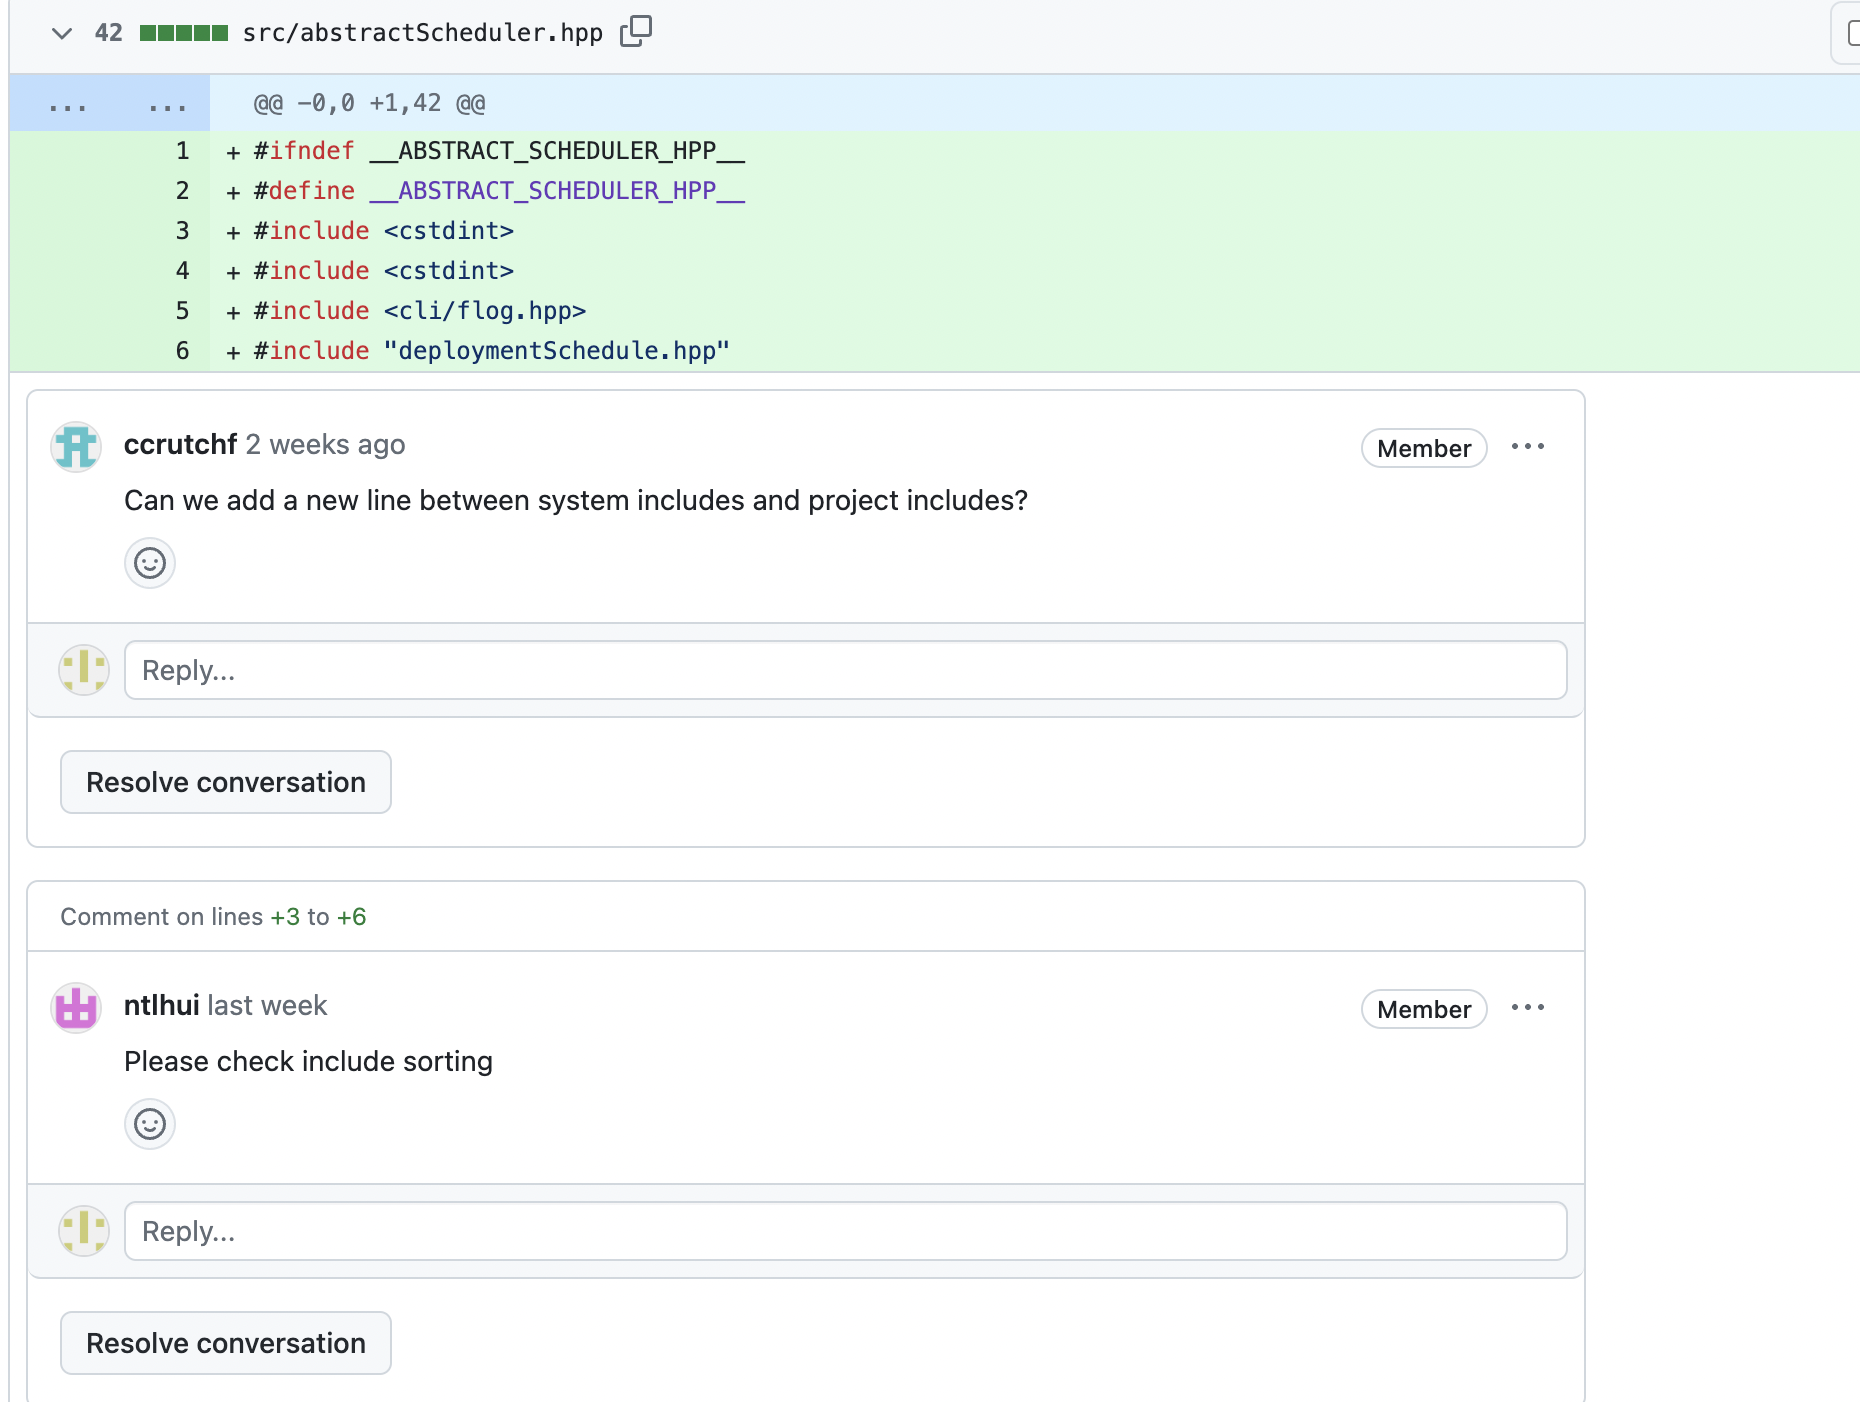
\includegraphics[height=1\textheight,width=1\textwidth,keepaspectratio]{images/commentsCodeReview.png}
        \end{column}
    \end{columns}
\end{frame}
